\documentclass[t,11pt]{beamer}

\usetheme{Madrid}
\usecolortheme{default}

% Packages
\usepackage[utf8]{inputenc}
\usepackage[T1]{fontenc}
\usepackage{xcolor}
\usepackage{listings}
\usepackage{hyperref}
\usepackage{tikz}
\usepackage{xspace}
\usepackage{textcomp}

% Define colors
\definecolor{darkblue}{rgb}{0.1, 0.2, 0.5}
\definecolor{codegray}{gray}{0.95}
\definecolor{codegreen}{rgb}{0, 0.6, 0}
\definecolor{codepurple}{rgb}{0.58, 0, 0.82}

% Code listings
\lstset{
  language=python,
  basicstyle=\ttfamily\small,
  backgroundcolor=\color{codegray},
  commentstyle=\color{codegreen},
  keywordstyle=\color{darkblue},
  stringstyle=\color{codepurple},
  breaklines=true,
  showstringspaces=false,
  frame=single,
  rulecolor=\color{gray}
}

% Custom commands
\newcommand{\lean}{\texttt{Lean 4}\xspace}
\newcommand{\python}{\texttt{Python}\xspace}
\newcommand{\pd}{Prisoner's Dilemma\xspace}

% Title page
\title{Open Source Game Theory}
\subtitle{Formal Verification of Bot Strategies in \pd}
\author{Your Name}
\institute{ETH Zurich}
\date{April 2026}

\begin{document}

% Title slide
\frame{\titlepage}

% Slide 2: Table of Contents
\begin{frame}
  \frametitle{Outline}
  \tableofcontents
\end{frame}

% Section 1: Motivation
\section{Motivation}

\begin{frame}
  \frametitle{Why Formal Verification for Game Theory?}
  
  \begin{itemize}
    \item Game-theoretic code is inherently complex
    \item Even simple strategies can have subtle bugs
    \item In multi-agent systems, correctness is critical
    \item Traditional testing may miss edge cases
  \end{itemize}
  
  \vspace{0.5cm}
  
  \textbf{Solution:} Combine formal verification with practical automation
\end{frame}

\begin{frame}
  \frametitle{The Challenge}
  
  \begin{columns}[T]
    \column{0.5\textwidth}
    \textbf{Traditional Approach:}
    \begin{itemize}
      \item Write strategy code
      \item Test manually
      \item Prove properties separately (if at all)
    \end{itemize}
    
    \column{0.5\textwidth}
    \textbf{Our Approach:}
    \begin{itemize}
      \item Formalize game semantics
      \item Auto-generate verification code
      \item Cache proven theorems
      \item Verify on-demand
    \end{itemize}
  \end{columns}
\end{frame}

% Section 2: Architecture
\section{Architecture}

\begin{frame}
  \frametitle{System Overview}
  
  \begin{center}
    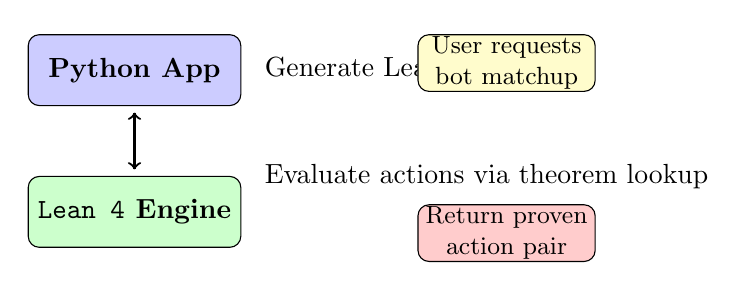
\begin{tikzpicture}[scale=0.9]
      \draw[rounded corners, fill=blue!20] (0, 3) rectangle (3, 4) node[pos=.5] {\textbf{Python App}};
      \draw[rounded corners, fill=green!20] (0, 1) rectangle (3, 2) node[pos=.5] {\textbf{\lean Engine}};
      
      \draw[->, thick] (1.5, 2.9) -- (1.5, 2.1);
      \draw[->, thick] (1.5, 2.1) -- (1.5, 2.9);
      
      \node[anchor=west] at (3.2, 3.5) {Generate Lean snippets};
      \node[anchor=west] at (3.2, 2) {Evaluate actions via theorem lookup};
      
      % Boxes for details
      \draw[rounded corners, fill=yellow!20] (5.5, 3.2) rectangle (8, 4);
      \node[align=center, font=\small] at (6.75, 3.6) {User requests\\bot matchup};
      
      \draw[rounded corners, fill=red!20] (5.5, 0.8) rectangle (8, 1.6);
      \node[align=center, font=\small] at (6.75, 1.2) {Return proven\\action pair};
    \end{tikzpicture}
  \end{center}
  
  \vspace{0.5cm}
  
  \begin{itemize}
    \item \textbf{Engine}: Formalize \pd semantics and prove action claims
    \item \textbf{App}: Orchestrate bot matchups and cache theorems
  \end{itemize}
\end{frame}

\begin{frame}[fragile]
  \frametitle{\lean Engine: Core Components}
  
  \begin{itemize}
    \item \textbf{Core.lean}: Game semantics and payoff matrix
    \begin{lstlisting}[basicstyle=\ttfamily\tiny]
structure Outcome where
  left: Action
  right: Action
    \end{lstlisting}
    
    \item \textbf{Pipeline.lean}: Program interaction model
    \begin{lstlisting}[basicstyle=\ttfamily\tiny]
theorem ActionClaim (left right: Bot) 
  (l r: Action) : Prop := 
  playActions left right = (l, r)
    \end{lstlisting}
    
    \item \textbf{Models/}: Bot definitions (CooperateBot, DefectBot, DBot, etc.)
    \item \textbf{Proofs/}: Proven ActionClaim theorems for key matchups
  \end{itemize}
\end{frame}

\begin{frame}[fragile]
  \frametitle{\python App: Theorem Discovery}
  
  \begin{lstlisting}[basicstyle=\ttfamily\footnotesize]
def discover_action_claim_theorems():
    """Scan Proofs folder for ActionClaim theorems"""
    pattern = r'theorem\s+(\w+_vs_\w+_actionClaim)'
    theorems = {}
    
    for lean_file in PROOFS_DIR.glob("*.lean"):
        for match in re.finditer(pattern, file_content):
            theorem_name = match.group(1)
            # Extract expected actions from theorem
            theorems[(left_bot, right_bot)] = \
              (theorem_name, action_l, action_r)
    
    return theorems
  \end{lstlisting}
  
  \small
  \begin{itemize}
    \item Automatically discovers all proven theorems at startup
    \item No manual configuration needed — add a proof, it's instantly available
  \end{itemize}
\end{frame}

% Section 3: Key Features
\section{Key Features}

\begin{frame}
  \frametitle{Feature 1: Dynamic Theorem Discovery}
  
  \begin{enumerate}
    \item User requests bot matchup
    \item App scans proofs for matching theorem
    \item If found: use proven result
    \item If not found: generate and prove on-the-fly
  \end{enumerate}
  
  \vspace{0.5cm}
  \textbf{Benefit:} No manual configuration — add a proof, it's instantly available
\end{frame}

\begin{frame}
  \frametitle{Feature 2: Symmetric Bot Pairings}
  
  \textbf{Problem:} Game theory is symmetric, but we only prove some theorem pairs
  
  \begin{center}
    \begin{tabular}{lcc}
      \hline
      \textbf{Request} & \textbf{Theorem} & \textbf{Actions} \\
      \hline
      oBot vs dBot & \texttt{oBot\_vs\_dBot} & (D, C) \\
      dBot vs oBot & \texttt{oBot\_vs\_dBot}* & (C, D)* \\
      \hline
    \end{tabular}
  \end{center}
  
  \small\vspace{0.3cm}
  \textbf{Solution:}
  \begin{enumerate}
    \item Detect if reverse-order theorem exists
    \item Evaluate it with swapped bot order
    \item Swap returned actions to match requested order
  \end{enumerate}
  
  \vspace{0.3cm}
  Result: Users don't care about proof direction — both orderings work!
\end{frame}

\begin{frame}[fragile]
  \frametitle{Feature 3: Automated Action Verification}
  
  Users can claim what actions a bot pair should produce:
  
  \vspace{0.3cm}
  
  \small
  \textbf{Prove true claim:}
  \begin{lstlisting}[basicstyle=\ttfamily\small]
$ uv run run-matchup --left dBot --right defectBot \
    --claim-left C --claim-right D
proof: PD.Proofs.DBot.dbot_vs_defect_actionClaim
  \end{lstlisting}
  
  \vspace{0.3cm}
  
  \textbf{Disprove false claim:}
  \begin{lstlisting}[basicstyle=\ttfamily\small]
$ uv run run-matchup --left dBot --right defectBot \
    --claim-left D --claim-right C
# Error: lean execution failed
  \end{lstlisting}
\end{frame}

% Section 4: Implementation Results
\section{Results}

\begin{frame}
  \frametitle{Current State: 24 Proven Theorems}
  
  \begin{center}
    \small
    \begin{tabular}{ll}
      \hline
      \textbf{Proof File} & \textbf{Theorems} \\
      \hline
      CooperateBot.lean & 3 \\
      DefectBot.lean & 3 \\
      DBot.lean & 7 \\
      OBot.lean & 2 \\
      MirrorBot.lean & 4 \\
      EBot.lean & 3 \\
      TitForTat.lean & 2 \\
      \hline
      \textbf{Total} & \textbf{24} \\
      \hline
    \end{tabular}
  \end{center}
  
  \vspace{0.5cm}
  \textbf{All discovered automatically} — app invokes dynamic scanning at startup
\end{frame}

\begin{frame}
  \frametitle{Test Suite: Full Coverage}
  
  \begin{center}
    \large
    \textbf{20/20 Tests Passing [OK]}
  \end{center}
  
  \vspace{0.3cm}
  
  \small
  \begin{itemize}
    \item \textbf{CLI tests}: Command parsing and output formatting
    \item \textbf{Theorem discovery}: Dynamic scanning \& reverse lookup
    \item \textbf{Action swapping}: Symmetric pairing verification
    \item \textbf{Lean integration}: Code generation and execution
  \end{itemize}
  
  \vspace{0.5cm}
  
  \textbf{Example:} Test validates that \texttt{dBot vs oBot} uses the reverse theorem and swaps actions correctly
\end{frame}

\begin{frame}[fragile]
  \frametitle{Live Demo}
  
  \textbf{Direct order:}
  \begin{verbatim}
$ uv run run-matchup --left oBot --right dBot
left bot:  oBot
right bot: dBot
actions:   (D, C)
proof:     PD.Proofs.OBot.oBot_vs_dBot_actionClaim
  \end{verbatim}
  
  \vspace{0.3cm}
  
  \textbf{Reversed order (automatic):}
  \begin{verbatim}
$ uv run run-matchup --left dBot --right oBot
left bot:  dBot
right bot: oBot
actions:   (C, D)
proof:     PD.Proofs.OBot.oBot_vs_dBot_actionClaim
  \end{verbatim}
  
  \small
  Same theorem, same correctness, user sees symmetric results!
\end{frame}

% Section 5: Conclusion
\section{Conclusion}

\begin{frame}
  \frametitle{Key Takeaways}
  
  \begin{itemize}
    \item \textbf{Formal verification} + \textbf{automation} = practical game theory proofs
    \vspace{0.3cm}
    \item \textbf{Dynamic discovery} eliminates configuration overhead
    \vspace{0.3cm}
    \item \textbf{Symmetric reasoning} makes the system user-friendly
    \vspace{0.3cm}
    \item \textbf{Proved theorems are cached} — instant verification for common matchups
  \end{itemize}
\end{frame}

\begin{frame}
  \frametitle{Future Work}
  
  \begin{itemize}
    \item Prove theorems for additional bot families (e.g., learning-based strategies)
    \vspace{0.3cm}
    \item Extend to $n$-player games beyond 2-player \pd
    \vspace{0.3cm}
    \item Auto-generate proofs for simple bots (always-cooperate, always-defect)
    \vspace{0.3cm}
    \item REST API for theorem verification as a service
    \vspace{0.3cm}
    \item Formal proof of the action-swapping algorithm itself
  \end{itemize}
\end{frame}

\begin{frame}
  \frametitle{Questions?}
  
  \begin{center}
    \large
    \vspace{1cm}
    Repository: \texttt{open-source-game-theory} \\
    \vspace{0.5cm}
    Engine: \lean 4 \\
    Orchestrator: \python \\
    \vspace{0.5cm}
    \textit{All tests passing. Ready for verification.}
  \end{center}
\end{frame}

\end{document}
